\section{Timeseries Prediction}

A time series is a sequence of observations, ordered in time.
Forecasting involves training a model on historical data and using them to predict future observations.
A simple example is a linear auto-regressive model.
The linear auto-regressive (AR) model of a time-series $Z_t$ with $t = 1,2,\dots,\infty$ is given by
\begin{equation*}
    \hat{z}_t = a_1 z_{t-1} + a_2 z_{t-2} + \dots + a_p z_{t-p} \enspace,
\end{equation*}
with $a_i \in \mathbb{R}$ for $i=1,\dots,p$ and $p$ the model lag.
The prediction for a certain time $t$ is equal to a weighted sum of the previous values up to a certain lag $p$.
In a similar way, the nonlinear variant (NAR) is described as
\begin{equation*}
    \hat{z}_t = f(z_{t-1},z_{t-2}, \dots,z_{t-p}) \enspace.
\end{equation*}

A depiction of this process can be found in Figure~\ref{fig:nar}.
Remark that in this way, the time-series identification can be written as a classical black-box regression modeling problem $\hat{y}_t = f(x_t)$, with $y_t = z_t$ and $x_t = [z_{t-1}, z_{t-2}, \dots, z_{t-p}]$.
When preparing the dataset and applying train/validation/test splits, it is important to prevent \emph{data leakage} by respecting the temporal information flow.
More precisely, a datapoint $z_t$ should not be part of two splits --- either as input $x_t$ or target $y_t$ --- and training (or validation) sets should not contain datapoints that occur after test datapoints.

\begin{figure}[h]
	\centering
	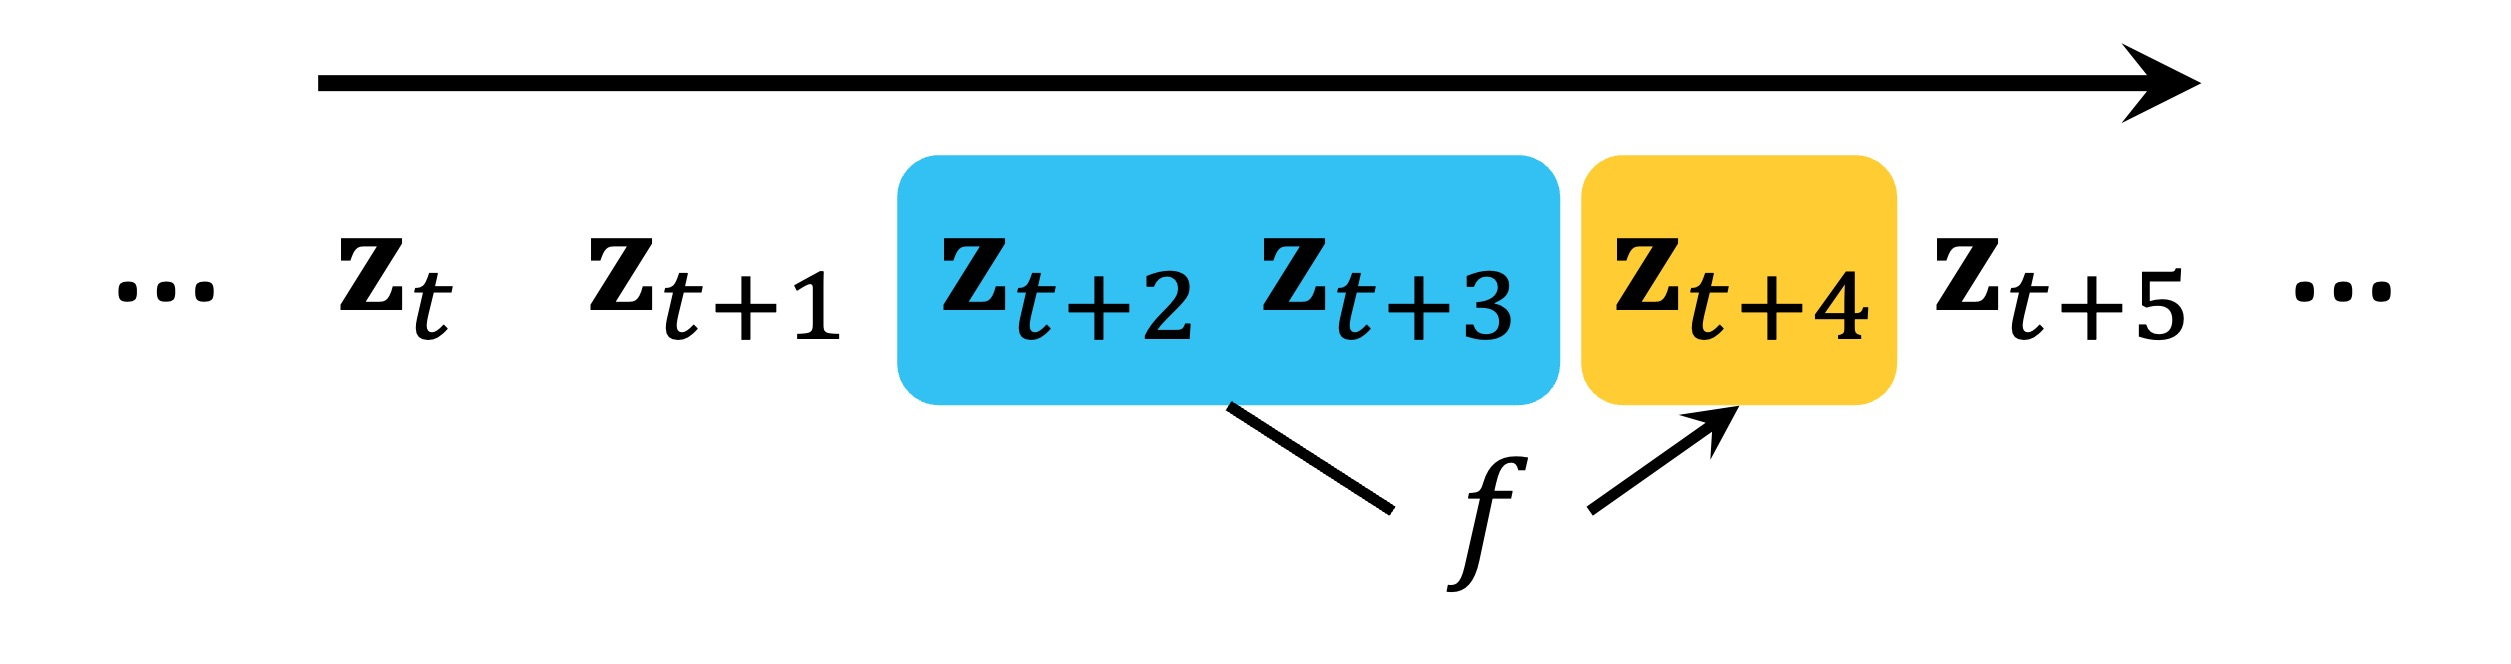
\includegraphics[width=0.6\textwidth]{images/nar.jpg}
	\caption{Schematic representation of the nonlinear auto-regressive model with lag $p=2$.}
	\label{fig:nar}
\end{figure}

\kulbox{To answer the questions in this section, you will need the notebook \texttt{time\_series.ipynb} that you can find on toledo, or alternatively using \href{https://colab.research.google.com/github/psanchezML/KUL_ANNDL_ExerciseSessions/blob/main/session2/time_series.ipynb}{this colab link}.}

%% ===================================================================
%%  ARCHITECTURE THEORY
%% ===================================================================

\subsection*{Recurrent Neural Networks (RNNs)}

A recurrent neural network \cite{Elman1990} processes a sequence element-by-element, maintaining a hidden state $\mathbf{h}_t$ that summarises all previously seen inputs:
\begin{align}
    \mathbf{h}_t &= \tanh\!\bigl(W_h\,\mathbf{h}_{t-1} + W_x\,\mathbf{x}_t + \mathbf{b}_h\bigr), \label{eq:rnn-hidden}\\
    \hat{y}_t &= W_y\,\mathbf{h}_t + b_y. \label{eq:rnn-output}
\end{align}
The key feature is \textbf{weight sharing}: the same matrices $W_h$, $W_x$ are applied at every time step, giving the model a strong inductive bias toward \emph{sequential processing} with translational equivariance in time.

% --- TikZ: unfolded RNN ---
\begin{figure}[h]
\centering
\begin{tikzpicture}[
    >=Stealth, node distance=14mm,
    cell/.style={draw, rounded corners, minimum width=12mm, minimum height=9mm, fill=blue!10, font=\small},
    io/.style={font=\small},
]
    \foreach \i in {1,2,3} {
        \node[cell] (h\i) at (2.5*\i, 0) {$\tanh$};
        \node[io, below=8mm of h\i] (x\i) {$x_{t\ifnum\i=1{-2}\fi\ifnum\i=2{-1}\fi\ifnum\i=3{}\fi}$};
        \node[io, above=8mm of h\i] (y\i) {$\hat{y}_{t\ifnum\i=1{-2}\fi\ifnum\i=2{-1}\fi\ifnum\i=3{}\fi}$};
        \draw[->] (x\i) -- (h\i);
        \draw[->] (h\i) -- (y\i);
    }
    \draw[->] (h1) -- node[above, font=\scriptsize]{$\mathbf{h}_{t\text{-}2}$} (h2);
    \draw[->] (h2) -- node[above, font=\scriptsize]{$\mathbf{h}_{t\text{-}1}$} (h3);
    \draw[->, dashed] (0.8,0) -- (h1);
    \draw[->, dashed] (h3) -- (10.2,0);
    \node[below=2mm of x2, font=\footnotesize, gray] {shared weights $W_h, W_x$};
\end{tikzpicture}
\caption{An RNN unfolded over three time steps. The same weights are reused at every step; the hidden state $\mathbf{h}_t$ carries temporal information forward.}
\label{fig:rnn-unfolded}
\end{figure}

\begin{insightbox}[title={The Vanishing Gradient Problem}]
During backpropagation through time (BPTT), gradients are multiplied by $W_h$ at each step.
If the spectral radius of $W_h$ is less than 1, gradients \emph{vanish} exponentially with sequence length; if greater than 1, they \emph{explode} \cite{VanishingGradient}.
This limits simple RNNs to learning dependencies over \textbf{short-to-moderate} time horizons.
\end{insightbox}

\subsection*{Long Short-Term Memory Network (LSTM)}

Long Short Term Memory networks \cite{LSTM} solve the vanishing gradient problem by introducing a \emph{cell state} $\mathbf{c}_t$ and three \emph{gates} that regulate information flow:
\begin{align}
    \mathbf{f}_t &= \sigma\!\bigl(W_f\,[\mathbf{h}_{t-1};\,\mathbf{x}_t] + \mathbf{b}_f\bigr) & &\text{(forget gate)} \label{eq:lstm-forget}\\
    \mathbf{i}_t &= \sigma\!\bigl(W_i\,[\mathbf{h}_{t-1};\,\mathbf{x}_t] + \mathbf{b}_i\bigr) & &\text{(input gate)} \label{eq:lstm-input}\\
    \tilde{\mathbf{c}}_t &= \tanh\!\bigl(W_c\,[\mathbf{h}_{t-1};\,\mathbf{x}_t] + \mathbf{b}_c\bigr) & &\text{(candidate)} \\
    \mathbf{c}_t &= \mathbf{f}_t \odot \mathbf{c}_{t-1} \;+\; \mathbf{i}_t \odot \tilde{\mathbf{c}}_t & &\text{(cell update)} \label{eq:lstm-cell}\\
    \mathbf{o}_t &= \sigma\!\bigl(W_o\,[\mathbf{h}_{t-1};\,\mathbf{x}_t] + \mathbf{b}_o\bigr) & &\text{(output gate)} \\
    \mathbf{h}_t &= \mathbf{o}_t \odot \tanh(\mathbf{c}_t) & &\text{(hidden state)} \label{eq:lstm-hidden}
\end{align}
where $\sigma$ is the sigmoid function, $\odot$ denotes element-wise multiplication, and $[\cdot\,;\,\cdot]$ is concatenation.

The cell state acts as a \textbf{conveyor belt}: the forget gate decides what to discard, the input gate decides what new information to write, and the output gate controls what to expose.
Because the cell state is updated via \emph{additive} interactions (Eq.~\ref{eq:lstm-cell}), gradients can flow across many time steps without vanishing, enabling LSTMs to capture \textbf{long-range dependencies}.

% --- TikZ: LSTM cell ---
\begin{figure}[h]
\centering
\begin{tikzpicture}[
    >=Stealth, scale=0.8, every node/.style={scale=0.8},
    gate/.style={draw, circle, inner sep=2pt, minimum size=7mm, font=\small},
    op/.style={draw, circle, inner sep=1pt, minimum size=6mm, font=\footnotesize},
    arr/.style={->, thick},
    block/.style={draw, rounded corners, minimum width=14mm, minimum height=7mm, fill=yellow!15, font=\small},
]
    % Cell state line
    \draw[arr, line width=1.5pt, blue!60] (-1,3) -- node[above, font=\footnotesize, black]{$\mathbf{c}_{t-1}$} (1.5,3);
    \node[op, fill=red!15] (forget) at (2.5,3) {$\times$};
    \node[op, fill=green!15] (add) at (5,3) {$+$};
    \draw[arr, line width=1.5pt, blue!60] (forget) -- (add);
    \draw[arr, line width=1.5pt, blue!60] (add) -- (8.5,3) node[right, black, font=\footnotesize]{$\mathbf{c}_t$};

    % Forget gate
    \node[block, fill=red!10] (fg) at (2.5,0.8) {$\sigma$};
    \draw[arr] (fg) -- node[right, font=\scriptsize]{$\mathbf{f}_t$} (forget);
    \node[font=\footnotesize, red!60!black] at (2.5,0) {forget};

    % Input gate + candidate
    \node[block, fill=green!10] (ig) at (4.2,0.8) {$\sigma$};
    \node[block, fill=blue!10] (cand) at (5.8,0.8) {$\tanh$};
    \node[op, fill=green!15] (imul) at (5,1.8) {$\times$};
    \draw[arr] (ig) -- (imul);
    \draw[arr] (cand) -- (imul);
    \draw[arr] (imul) -- (add);
    \node[font=\footnotesize, green!50!black] at (4.2,0) {input};

    % Output gate
    \node[block, fill=orange!10] (og) at (7.2,0.8) {$\sigma$};
    \node[op, fill=orange!15] (omul) at (7.2,2.2) {$\times$};
    \node[block, fill=blue!10] (otanh) at (6.2,2.2) {$\tanh$};
    \draw[arr] (og) -- node[right, font=\scriptsize]{$\mathbf{o}_t$} (omul);
    \draw[arr] (6.2,3) -- (otanh);
    \draw[arr] (otanh) -- (omul);
    \draw[arr] (omul) -- (8.5,2.2) node[right, font=\footnotesize]{$\mathbf{h}_t$};
    \node[font=\footnotesize, orange!60!black] at (7.2,0) {output};

    % Inputs
    \node[font=\footnotesize] at (0.5,-0.5) {$[\mathbf{h}_{t-1};\,\mathbf{x}_t]$};
    \draw[arr, dashed] (0.5,-0.2) -- (0.5,0.8) -| (fg);
    \draw[dashed] (0.5,0.8) -| (ig);
    \draw[dashed] (0.5,0.8) -| (cand);
    \draw[dashed] (0.5,0.8) -| (og);
\end{tikzpicture}
\caption{LSTM cell architecture.  The cell state $\mathbf{c}_t$ (blue line) flows left to right, modulated by the forget gate ($\times$, red) and enriched by the input gate ($+$, green).  The output gate (orange) controls the exposed hidden state.}
\label{fig:lstm-cell}
\end{figure}


\subsection*{Multilayer Perceptron for Time Series}

The MLP treats time-series prediction as a \emph{static regression} problem.
The input is a fixed window of $p$ past values $[z_{t-1}, \dots, z_{t-p}]$ and the output is the prediction $\hat{z}_t$.
The training is done in feedforward mode:
\begin{equation}
    \hat{z}_{t} = w^\top\tanh(V [z_{t-1} ; z_{t-2}; ...; z_{t-p}] + \beta).
\end{equation}
In order to make predictions, the trained network is used in an iterative way as a recurrent network:
\begin{equation}
    \hat{z}_{t} = w^\top\tanh(V [\hat{z}_{t-1} ; \hat{z}_{t-2}; ...; \hat{z}_{t-p}] + \beta).
\end{equation}

% --- TikZ: sliding window ---
\begin{figure}[h]
\centering
\begin{tikzpicture}[>=Stealth, scale=0.75, every node/.style={scale=0.75}]
    % Time series
    \foreach \i in {0,...,11} {
        \pgfmathsetmacro{\yv}{1.5+0.8*sin(40*\i)+0.3*cos(80*\i)}
        \fill[blue!50] (\i*0.7, 0) circle (2pt);
        \ifnum\i>0
            \pgfmathsetmacro{\yprev}{1.5+0.8*sin(40*(\i-1))+0.3*cos(80*(\i-1))}
        \fi
    }
    \draw[thick, blue!60, smooth] plot coordinates {
        (0,1.5) (0.7,1.83) (1.4,2.08) (2.1,2.15) (2.8,2.02) (3.5,1.73)
        (4.2,1.38) (4.9,1.12) (5.6,1.02) (6.3,1.12) (7.0,1.38) (7.7,1.73)
    };

    % Window
    \draw[thick, red!70, fill=red!10, rounded corners=2pt]
        (2.8-0.25,-0.35) rectangle (5.6+0.25,0.35);
    \node[below, red!70!black, font=\footnotesize] at (4.2,-0.45) {lag window $p=4$};

    % Target
    \draw[->, thick, green!50!black] (5.6,0) -- (6.3,0);
    \fill[green!50!black] (6.3,0) circle (3pt);
    \node[above, green!50!black, font=\footnotesize] at (6.3,0.25) {target $z_t$};

    % Arrow to MLP
    \draw[->, thick] (4.2,-0.8) -- (4.2,-1.6) node[midway, right, font=\footnotesize] {input};
    \node[draw, rounded corners, fill=gray!10, minimum width=25mm, minimum height=8mm] at (4.2,-2.0) {MLP};
    \draw[->, thick] (4.2,-2.4) -- (4.2,-3.0) node[below, font=\footnotesize] {$\hat{z}_t$};
\end{tikzpicture}
\caption{The MLP approach: a sliding window of $p$ past values is fed as a fixed-size input vector.  The temporal structure is encoded \emph{only} through the lag embedding.}
\label{fig:mlp-sliding-window}
\end{figure}

To format the timeseries for training, you can use the provided function \texttt{prepare\_timeseries}.
Make sure you understand what this function does by trying it out on a small toy example.
To make predictions, a \texttt{for} loop needs to be implemented that includes the predicted value from the previous timestep in the input vector to predict the next timestep.
As this is a stateful model, make sure to reset the internal state using the \texttt{reset\_states} function before making new predictions.

\subsection*{Inductive Biases of Sequential Models}

\begin{insightbox}[title={Why does architecture matter?}]
Different architectures impose different \emph{inductive biases}---implicit assumptions about the data:
\begin{itemize}
    \item \textbf{MLP}: assumes all relevant information is within a \emph{fixed window} of $p$ past values.  No notion of sequential order beyond position in the input vector.  Works best when the system has \textbf{strong local structure} and a well-defined lag.
    \item \textbf{Simple RNN}: assumes \emph{sequential processing} with shared weights at each step.  The hidden state carries a compressed summary of the past.  Excels at \textbf{moderate-range periodic} patterns but struggles with very long dependencies due to vanishing gradients.
    \item \textbf{LSTM}: adds \emph{selective memory} through gating.  Can learn to remember information over hundreds of steps.  Best suited for data with \textbf{long-range dependencies} that simpler models cannot capture.
\end{itemize}
Choosing the right architecture requires understanding the \emph{temporal structure} of your data---which is why exploratory data analysis (autocorrelation, spectral analysis) is so valuable before modelling.
\end{insightbox}


%% ===================================================================
%%  DATASETS
%% ===================================================================

\subsection*{Santa Fe Laser Dataset}
The Santa Fe laser dataset is obtained from a chaotic laser which can be described as a nonlinear dynamical system.
The first $1000$ data points can be used for training and validation purposes.
The aim is to predict the next $100$ points (it is forbidden to include these points in the training or validation sets!).
Both datasets are stored in \texttt{SantaFe.npz} and are shown in Figure~\ref{fig:santafe}.
Before training any of the models, it is important to normalize the data, such that it has zero mean and unit variance.

This dataset has \textbf{strong local nonlinear structure}: the value at time $t$ is largely determined by a short window of recent values.
An MLP with a well-chosen lag can capture this mapping directly and efficiently, without the overhead of sequential processing.

\begin{figure}[h]
	\centering
	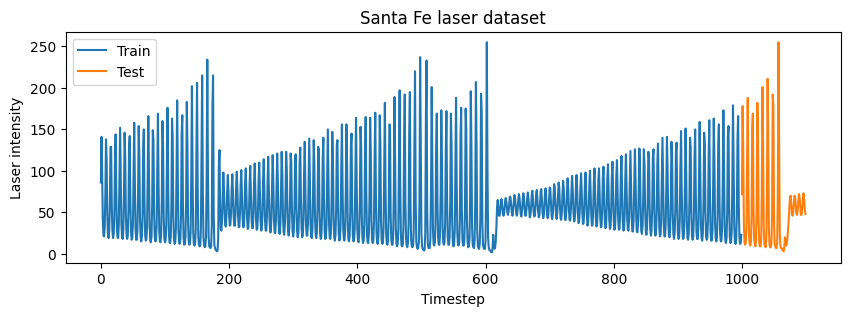
\includegraphics[width=0.9\textwidth]{images/santafe.png}
	\caption{Visualization of the Santa Fe laser dataset.}
	\label{fig:santafe}
\end{figure}

\subsection*{Mackey-Glass Time Series}
The Mackey-Glass equation \cite{MackeyGlass} is a delay differential equation originally proposed to model physiological control systems:
\begin{equation}
    \frac{dx}{dt} = \frac{\beta\, x(t-\tau)}{1 + x(t-\tau)^n} - \gamma\, x(t),
\end{equation}
with typical parameters $\beta=0.2$, $\gamma=0.1$, $n=10$.
The delay parameter $\tau$ controls the complexity: for $\tau > 17$ the system becomes chaotic.

With $\tau = 30$, the current value depends on information from \textbf{30 time steps in the past}, creating genuine long-range dependencies.
Simple RNNs suffer from vanishing gradients over these spans, making this the ideal dataset to demonstrate the advantage of \textbf{LSTMs}, whose gating mechanism can selectively preserve information across long horizons.

\subsection*{Sunspot Numbers}
Monthly sunspot counts have been recorded for over 300~years, making this one of the oldest scientific time series.
The data exhibits a prominent $\sim$11-year cycle (approximately 132~months) with varying amplitude and shape from cycle to cycle.

The regularity of the cycle means that the hidden state of a \textbf{simple RNN} can naturally track the phase of the oscillation, giving it an edge over MLPs (which would require an impractically large lag to see a full cycle) while not needing the heavy gating of an LSTM (since the relevant dependencies are moderate in length and the pattern is quasi-periodic).

\kulbox{Explore all three datasets interactively with the \textbf{Time Series Model Comparison} demo in \texttt{demos/timeseries\_explorer/}.
It provides EDA tools, side-by-side model training, and detailed ablation comparisons.
Run with: \texttt{streamlit run demos/timeseries\_explorer/app.py}}

%% ===================================================================
%%  EXERCISES
%% ===================================================================
\subsection*{Exercises}
\begin{questions}
    \item Train an MLP with one hidden layer on the \textbf{Santa Fe} dataset.
    Investigate the model performance with different lags and number of neurons.
    Discuss how the model looks and explain clearly how you tune the parameters and what the influence on the final prediction is.
    Which combination of parameters gives the best performance (MSE) on the test set?
	\item Do the same for the LSTM model and explain the design process.
    What is the effect of changing the lag value for the LSTM network?
	\item Compare the results of the recurrent MLP with the LSTM. Which model do you prefer and why?

    %% --- NEW EXERCISES ---
    \item \textbf{Ablation Study Across Datasets.}\;
    Train an MLP, a Simple RNN, and an LSTM on \emph{all three} datasets (Santa Fe, Mackey-Glass with $\tau{=}30$, Sunspot numbers).
    For each model--dataset pair:
    \begin{itemize}
        \item Report the test MSE and plot the predicted vs.\ actual time series.
        \item Create a summary table (3 models $\times$ 3 datasets).
        \item Discuss which model performs best on each dataset and \emph{why}, relating your observations to the inductive biases described above and to the data characteristics you discover in Exercise~5.
    \end{itemize}
    Ensure the comparison is fair: use the same lag, training budget, and validation strategy across models for each dataset.

    \item \textbf{Time Series EDA and Feature Analysis.}\;
    Before fitting any model, perform an exploratory data analysis on each of the three datasets:
    \begin{itemize}
        \item Plot the raw time series with rolling mean and standard deviation.
        \item Compute and plot the autocorrelation (ACF) and partial autocorrelation (PACF) functions.
        \item Estimate the spectral density to identify dominant frequencies.
        \item Run an Augmented Dickey-Fuller (ADF) test for stationarity.
    \end{itemize}
    Use the results to justify your choice of lag $p$ for each dataset and discuss what the ACF/PACF tell you about the nature of each time series (short-range vs.\ long-range dependencies, periodicity, trend).
\end{questions}
